\documentclass[titlepage,11pt]{article}
\usepackage{comment}
\usepackage{enumitem}
\usepackage{transparent} % Untuk transparansi gambar
\usepackage{listings}
\usepackage{amsmath}
\usepackage{graphicx}
\usepackage[font=small,labelfont=bf]{caption}
\usepackage[bahasa]{babel}
\usepackage{float}
\usepackage{verbatim}
\usepackage{graphicx,tabularx,multirow}
\usepackage{xcolor}
\usepackage[onehalfspacing]{setspace}
\usepackage[
	allcolors=visigrey,
	colorlinks=true,
]{hyperref}
\usepackage[a4paper,left=2cm,right=2cm]{geometry}
% Pengaturan kutipan artikel
\usepackage[style=ieee, backend=biber]{biblatex}
%Code listing style pak akok
\definecolor{codegreen}{rgb}{0,0.6,0}
\definecolor{codegray}{rgb}{0.5,0.5,0.5}
\definecolor{codepurple}{rgb}{0.58,0,0.82}
\definecolor{backcolour}{rgb}{0.95,0.95,0.92}

\usepackage{eso-pic} % Untuk menambahkan elemen ke seluruh halaman

\newcommand\BackgroundPic{
  \put(0,0){
    \parbox[b][\paperheight]{\paperwidth}{
      \vfill
      \centering
      \transparent{0.1}
      \includegraphics[width=0.4\paperwidth,keepaspectratio]{miot.png}
      \vfill
    }
  }
}

\newcommand\BackgroundAllPages{ \AddToShipoutPicture*{\BackgroundPic} }
\newcommand\BackgroundNone{ \ClearShipoutPicture } % hilangkan background

\lstdefinestyle{mystyle}{
	backgroundcolor=\color{backcolour}, commentstyle=\color{codegreen},
	keywordstyle=\color{magenta},
	numberstyle=\small\color{codegray},
	stringstyle=\color{codepurple},
	basicstyle=\ttfamily\footnotesize,
	breakatwhitespace=false,         
	breaklines=true,                 
	captionpos=t,                    
	keepspaces=true,                 
	numbers=left,                    
	numbersep=5pt,                  
	showspaces=false,                
	showstringspaces=false,
	showtabs=false,           
	frame = single,
	tabsize=2
}
\lstset{style=mystyle}

\definecolor{visigrey}{rgb}{.1,.15,.15}
\geometry{top=1cm,bottom=.5cm}
\savegeometry{titlepage}
\geometry{top=2cm,bottom=2cm}
\savegeometry{main}

\def\bspace{\(\qquad\qquad\qquad\)}
\usepackage[T1]{fontenc}
\usepackage[utf8]{inputenc}
\usepackage{tgheros}
\renewcommand*\familydefault{\sfdefault}

\setcounter{tocdepth}{6}

\def\autor{Laboratorium }
\def\lab{Multimedia dan Internet of Things}
\def\departemen{Departemen Teknik Komputer}
\def\institut{Institut Teknologi Sepuluh Nopember}
\def\praktikum{Laporan Sementara \\ Praktikum Jaringan Komputer}
\def\nama{Abraham Napitupulu - 5024231048}
% Ubah Judul sesuai dengan modul
\def\judul{Jaringan Nirkabel}
\def\tanggal{2025}
\begin{document}
% Ubah Bahasa sesuai dengan keinginan
\selectlanguage{bahasa}

\BackgroundNone
\def\headingtype{\bf \small}
\loadgeometry{titlepage}

\begin{titlepage}
	\centering
	\begin{tabularx}{\textwidth}{l@{\hskip 0pt}lX}
		\raisebox{-0.5\height}{
\includegraphics[width=3cm]{Cover/img/logodepart.png}} 
		& \raisebox{-0.5\height}{\includegraphics[width=3cm]{Cover/img/miot.png}} 
		& \raggedleft
	\hfill
	\begin{minipage}{0.5\textwidth}
		\raggedleft
		{\emph{\headingtype \autor}} \\[-2pt]
		{\headingtype \lab} \\[-2pt]
		{\headingtype \departemen} \\[-2pt]
		{\headingtype \emph{\institut}}
	\end{minipage}

	\vspace{5cm}
	\end{tabularx}
	
	\vspace{5cm}
	{\Huge \bf \praktikum \par}
	
	\vspace{2cm}
	{\LARGE \bf \judul \par}
	
	\vspace{2cm}
	{\Large \nama \par}
	
	\vfill
	{\Large \tanggal \par}
	
	\vfill
	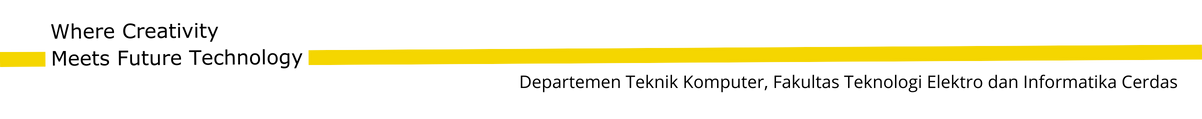
\includegraphics[width=\textwidth]{Cover/img/footer.png}
\end{titlepage}

\loadgeometry{main}


\BackgroundAllPages
% Pilih Modul yang akan di build
\section{Pendahuluan}
\subsection{Latar Belakang}
Jaringan wireless, atau jaringan nirkabel, adalah jenis jaringan komunikasi yang memungkinkan perangkat terhubung tanpa menggunakan kabel. Sebagai pengganti kabel, jaringan ini memanfaatkan gelombang elektromagnetik seperti gelombang radio atau inframerah untuk mentransmisikan data. Konsep ini bisa dianalogikan dengan perbedaan antara jalan raya yang memerlukan konstruksi fisik (kabel) dan udara yang bebas dilalui sinyal (wireless), yang menawarkan fleksibilitas dan mobilitas lebih besar bagi penggunanya. Salah satu jenis jaringan wireless yang paling umum adalah Wi-Fi, yang memungkinkan perangkat seperti komputer dan smartphone terhubung ke internet tanpa kabel melalui gelombang radio. Keberadaan Wi-Fi memudahkan pengguna untuk mengakses internet hanya dengan memilih jaringan dan memasukkan kata sandi, tanpa perlu kabel fisik yang terhubung. Selain itu, Bluetooth juga merupakan teknologi wireless yang lebih fokus pada koneksi perangkat jarak pendek, seperti menghubungkan ponsel ke speaker atau printer tanpa kabel. Bluetooth umumnya lebih hemat daya dan tidak memerlukan router atau access point seperti Wi-Fi. Meskipun keduanya menggunakan gelombang radio, Wi-Fi lebih cocok untuk akses internet dengan jangkauan lebih luas, sedangkan Bluetooth ideal untuk komunikasi antar perangkat dalam jarak dekat. Teknologi jaringan wireless ini sangat penting dalam dunia modern karena memberikan kemudahan dalam mobilitas dan efisiensi pengelolaan perangkat jaringan, baik di rumah, kantor, maupun ruang publik.
\subsection{Dasar Teori}
Jaringan wireless adalah sistem komunikasi yang memungkinkan perangkat untuk terhubung dan berkomunikasi tanpa menggunakan kabel fisik. Sebagai pengganti kabel, jaringan wireless memanfaatkan gelombang elektromagnetik seperti gelombang radio atau inframerah sebagai media transmisi data. Konsep ini memberikan fleksibilitas yang lebih besar dibandingkan dengan jaringan kabel, yang mengharuskan perangkat tetap terhubung secara fisik. Dalam jaringan wireless, sinyal dapat mengalir melalui udara, menghubungkan perangkat tanpa hambatan fisik, yang memungkinkan mobilitas dan efisiensi dalam pengelolaan perangkat jaringan.
Salah satu jenis jaringan wireless yang paling populer adalah Wi-Fi (Wireless Fidelity). Wi-Fi merupakan standar untuk jaringan Wireless Local Area Network (WLAN) yang menghubungkan perangkat seperti komputer, smartphone, dan perangkat lainnya ke internet tanpa kabel. Wi-Fi menggunakan gelombang radio untuk mentransmisikan data pada kecepatan tinggi, memungkinkan perangkat untuk mengakses internet melalui router wireless. Router Wi-Fi bertindak sebagai pusat penghubung antara perangkat lokal dan internet, dengan memancarkan sinyal Wi-Fi ke area sekitarnya, yang dapat diakses oleh perangkat yang terhubung.
Selain Wi-Fi, Bluetooth juga merupakan teknologi wireless yang lebih fokus pada komunikasi perangkat jarak pendek. Bluetooth memungkinkan perangkat seperti ponsel, speaker, dan printer untuk saling terhubung tanpa kabel dalam jangkauan yang lebih dekat, umumnya kurang dari 10 meter. Teknologi ini menggunakan frekuensi 2.4 GHz yang juga digunakan oleh Wi-Fi, namun dengan tujuan yang berbeda—untuk menghubungkan perangkat secara langsung (peer-to-peer) tanpa memerlukan router atau access point. Bluetooth lebih hemat daya dibandingkan Wi-Fi, menjadikannya pilihan ideal untuk perangkat yang membutuhkan komunikasi jarak dekat, seperti transfer file atau koneksi audio.
Meskipun Wi-Fi dan Bluetooth menggunakan gelombang radio untuk mentransmisikan data, keduanya memiliki perbedaan signifikan dalam hal tujuan, jangkauan, kecepatan, dan daya yang digunakan. Wi-Fi lebih cocok untuk akses internet dengan jangkauan yang lebih luas dan kecepatan yang lebih tinggi, sedangkan Bluetooth lebih mengutamakan efisiensi daya dan koneksi antar perangkat dalam jarak dekat. Dengan berkembangnya teknologi wireless, kedua jenis jaringan ini telah menjadi elemen penting dalam kehidupan sehari-hari, memberikan kenyamanan dan kemudahan dalam menghubungkan perangkat tanpa keterbatasan kabel.
\section{Tugas Pendahuluan}
\begin{enumerate}
    \item \textbf{Mobilitas dan Fleksibilitas}
    Wireless: Jaringan nirkabel memberikan keuntungan besar dalam hal mobilitas dan fleksibilitas. Pengguna dapat bergerak bebas tanpa terbatas oleh kabel fisik. Ini sangat ideal untuk perangkat mobile seperti smartphone, laptop, tablet, dan perangkat lain yang sering dipindahkan, serta untuk pengaturan di ruang publik atau area yang membutuhkan koneksi internet di berbagai lokasi.
    Wired: Jaringan berkabel tidak memungkinkan mobilitas yang sama, karena perangkat harus tetap terhubung dengan kabel fisik. Hal ini lebih cocok untuk perangkat yang berada di tempat tetap seperti desktop di kantor, server di data center, atau sistem yang memerlukan koneksi stabil dan cepat tanpa gangguan.
    \textbf{Kecepatan dan Kestabilan}
    Wireless: Meskipun Wi-Fi dapat menawarkan kecepatan yang cukup tinggi, terutama pada standar terbaru seperti 802.11ac atau 802.11ax, kecepatan dan kestabilan sinyal sangat tergantung pada banyak faktor, seperti jarak dari router, hambatan fisik (tembok, dinding), dan interferensi dari perangkat lain yang menggunakan gelombang radio. Kecepatan bisa menurun signifikan jika jarak perangkat terlalu jauh dari router atau ada banyak hambatan.
    Wired: Jaringan berkabel, seperti Ethernet, memberikan koneksi yang sangat stabil dan cepat. Koneksi Ethernet umumnya lebih andal dan memiliki kecepatan yang lebih tinggi dibandingkan dengan Wi-Fi, serta tidak terpengaruh oleh interferensi atau jarak. Ini menjadikannya pilihan terbaik untuk kebutuhan yang membutuhkan kestabilan tinggi, seperti di laboratorium, pusat data, atau kantor yang membutuhkan koneksi internet yang sangat cepat dan stabil.
    \textbf{Kemudahan Pemasangan}
    Wireless: Pemasangan jaringan wireless jauh lebih praktis karena tidak memerlukan instalasi kabel fisik di seluruh area. Pengguna hanya perlu menghubungkan perangkat ke SSID Wi-Fi dan memasukkan kata sandi untuk mendapatkan akses. Ini membuatnya lebih cocok untuk penggunaan rumahan, ruang kerja yang lebih fleksibel, dan tempat umum seperti kafe atau bandara.
    Wired: Pemasangan jaringan berkabel lebih rumit karena memerlukan pemasangan kabel fisik, yang sering kali memakan waktu dan biaya lebih tinggi, terutama dalam jaringan yang lebih besar atau kompleks. Kabel harus ditarik ke berbagai titik, dan perlu mempertimbangkan penataan kabel agar tidak mengganggu estetika atau mobilitas.
    \textbf{Keamanan}
    Wireless: Jaringan wireless rentan terhadap ancaman keamanan seperti peretasan atau penyadapan, terutama jika tidak dilindungi dengan protokol keamanan yang tepat seperti WPA2 atau WPA3. Sinyal Wi-Fi yang dipancarkan dapat dengan mudah diakses oleh pihak yang tidak berwenang dalam jangkauan sinyal.
    Wired: Jaringan berkabel lebih aman secara fisik karena akses hanya bisa dilakukan melalui kabel yang terhubung langsung. Tidak ada sinyal yang dapat dipancarkan dan diakses dari jarak jauh, sehingga lebih sulit bagi peretas untuk mengakses data. Keamanan lebih terjamin, terutama dalam lingkungan yang sangat sensitif seperti data center atau kantor yang menangani informasi penting.        
    \textbf{Biaya}
    Wireless: Jaringan wireless umumnya lebih murah dalam hal instalasi awal karena tidak memerlukan kabel fisik. Namun, biaya untuk perangkat tambahan seperti router wireless yang lebih canggih dapat meningkatkan pengeluaran.
    Wired: Meskipun pemasangan jaringan berkabel memerlukan biaya awal yang lebih tinggi untuk instalasi kabel dan perangkat keras (seperti switch atau hub), biaya operasional dan pemeliharaan cenderung lebih rendah dalam jangka panjang, terutama karena kabel lebih stabil dan tidak terpengaruh oleh faktor eksternal seperti interferensi.
    \textbf{Lingkungan Penggunaan}
    Wireless: Jaringan nirkabel lebih cocok untuk penggunaan rumah, kantor kecil, kafe, bandara, dan tempat umum yang memerlukan konektivitas fleksibel tanpa tergantung pada kabel. Ini juga ideal untuk perangkat yang memerlukan mobilitas tinggi.
    Wired: Jaringan berkabel lebih ideal untuk lingkungan yang memerlukan kecepatan tinggi dan stabilitas, seperti di laboratorium komputer, pusat data, kantor besar, atau rumah dengan pengaturan perangkat tetap yang membutuhkan koneksi internet tanpa gangguan atau penurunan kecepatan.

    \item 
    \textbf{Modem} Modem (Modulator-Demodulator) menghubungkan jaringan rumah atau kantor ke internet melalui penyedia layanan internet (ISP). Modem mengubah sinyal digital dari perangkat menjadi sinyal analog dan sebaliknya. Tanpa modem, tidak ada koneksi ke internet, tetapi modem hanya menghubungkan satu perangkat ke internet.
    \textbf{Router} Router menghubungkan perangkat di jaringan lokal (LAN) dan mengarahkan lalu lintas data antara perangkat serta ke internet. Router bekerja dengan modem untuk membagikan koneksi internet ke banyak perangkat melalui kabel (Ethernet) atau nirkabel (Wi-Fi).
    \textbf {Access Point (AP)} Access Point memperluas cakupan jaringan Wi-Fi dalam area yang lebih luas. AP memungkinkan perangkat wireless untuk terhubung ke jaringan lokal yang dikelola oleh router, tanpa menyediakan koneksi langsung ke internet. Biasanya digunakan untuk memperluas jangkauan Wi-Fi di gedung atau area besar.

    \item 
    \textbf{Wireless Bridge}
    Tanpa Kabel: Wireless bridge memungkinkan transmisi data antar ruangan tanpa memerlukan kabel fisik, menggunakan sinyal Wi-Fi. Ini sangat praktis ketika pemasangan kabel sulit atau tidak memungkinkan.

    Jangkauan Lebih Jauh: Perangkat wireless bridge atau access point P2P dirancang untuk menghubungkan dua lokasi yang terpisah oleh jarak yang cukup jauh. Beberapa model dapat mencakup jangkauan beberapa ratus meter, tergantung pada kekuatan sinyal dan teknologi yang digunakan.

    Pengaturan Fleksibel: Anda dapat menempatkan access point di posisi strategis untuk memastikan sinyal yang optimal antara kedua ruangan. Cukup dengan memasang dua access point yang terhubung melalui sinyal Wi-Fi yang aman.

    Kualitas Sinyal Tinggi: Dengan penggunaan frekuensi 5 GHz atau teknologi yang lebih maju (seperti 802.11ac/ax), wireless bridge dapat memberikan kecepatan yang cukup tinggi untuk transmisi data antar dua lokasi tanpa kabel, lebih stabil daripada jaringan Wi-Fi biasa.

    Biaya dan Instalasi Lebih Rendah: Dibandingkan dengan instalasi kabel fisik yang memerlukan waktu dan biaya tinggi, menggunakan wireless bridge lebih ekonomis dan mudah dipasang.
\end{enumerate}

\end{document}